\noindent
\begin{tabular}{cc}
\begin{minipage}{0.60\textwidth}
\begin{exerciseS}[Motore a getto]
    Il motore a getto in figura è alimentato con una portata $\dot{m}_c = 
1.1\ kg/s$ di carburante liquido iniettato in direzione 
ortogonale all'asse del motore. Calcolare la spinta $T$ del 
motore ipotizzando che:
\begin{itemize}
\item il carburante vaporizzi e diffonda completamente;
\item le sezioni di ingresso e uscita abbiano area uguale e pari 
      ad $A = 0.5\ m^2$;
\item sia l'aria in ingresso che i gas di scarico siano a pressione 
    atmosferica $P_{atm}=26400\ Pa$;
\item la velocità di ingresso e di uscita siano uniformi sulle 
      rispettive sezioni;
\item siano note la densità dell'aria in ingresso $\rho_1 = 0.42\, 
      kg/m^3$, la velocità di ingresso $V_1 = 240\ m/s$ 
      e la velocità di efflusso $V_2 = 980\ m/s$.
\end{itemize}
($T = -38374\hat{\bm{x}}\ N$)
\end{exerciseS}
\end{minipage}
&
\begin{minipage}{0.35\textwidth}
   \begin{center}
   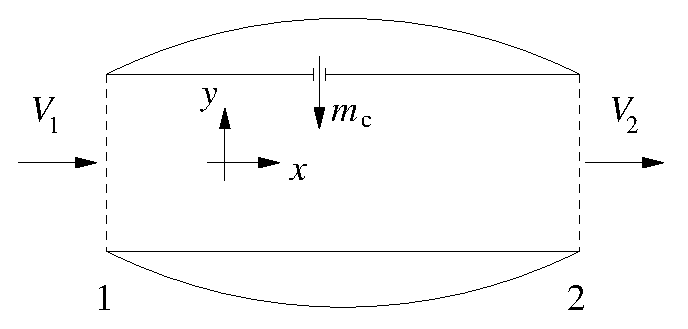
\includegraphics[width=0.90\textwidth]{./fig/motore_a_getto.eps}
   \end{center}
\end{minipage}
\end{tabular}

\sol
\begin{equation}
    T = \rho V_1 A (V_2-V_1) + V_2 \dot{m}_c \ .
\end{equation}

\partone
 Bilanci integrali di massa e quantità di moto.
\begin{equation}
\begin{cases}
  \frac{d}{dt} \int_V \rho = -\oint_{\partial V} \rho \bm{u} \cdot \hat{\bm{n}}  & \text{(massa)} \\
  \frac{d}{dt} \int_V \rho \bm{u} = -\oint_{\partial V} \rho \bm{u} \bm{u} \cdot \hat{\bm{n}}
  +\int_V \bm{f} - \oint_{\partial V} p \hat{\bm{n}} + \oint_{\partial V} \bm{s_n} & \text{(quantità di moto)}
\end{cases}
\end{equation}

\parttwo
Ipotesi: Regime stazionario. Fluido non viscoso (?). Profilo costante di velocità. No gravità.

\begin{itemize}
  \item Scrittura dei bilanci integrali con le semplificazioni opportune, derivanti dalle ipotesi.
    \begin{equation}
     \begin{cases}
      \oint_{\partial V} \rho \bm{u} \cdot \hat{\bm{n}} = 0  & \text{(massa)} \\
      \oint_{\partial V} \rho \bm{u} \bm{u} \cdot \hat{\bm{n}} = \oint_{\partial V} \bm{t_n} & \text{(quantità di moto)}
     \end{cases}
    \end{equation}
  \item Ulteriore semplificazione usando l'ipotesi di profili di velocità uniformi
    \begin{equation}
     \begin{cases}
      - \rho_1 V_1 A_1 -\dot{m}_c + \rho_2 V_2 A_2 = 0  \\
      - \rho_1 \vec{V_1} V_1 A_1 + \rho_2 \vec{V_2} V_2 A_2 - \dot{m}_c \vec{v}_c = \oint_{S1\cup S2\cup S3} \bm{t_n}
     \end{cases}
    \end{equation}
  \item Relazione tra l'integrale della pressione e la risultante delle forze agenti sul gomito, sfruttando il fatto che l'integrale della normale su tutta la superficie è identicamente nullo. Si identificano con $S_1$ la superficie di ingresso, $S_2$ la superficie di uscita, $S_3$ la superficie laterale interna del motore, $S_{3_o}$ la superficie laterale esterna del motore.
    \begin{equation}
     \begin{aligned}
      \displaystyle\oint_{S_1\cup S_2\cup S_3} \bm{t_n} & = \displaystyle\oint_{S_1\cup S_2\cup S_3} \bm{t_n} + \underbrace{\displaystyle\oint_{S_1\cup S_2\cup S{3_o}} p_a \hat{\bm{n}}}_{=0} = \\
      & = -\int_{S_1} (p-p_a) \hat{\bm{n}} - \int_{S_2} (p-p_a) \hat{\bm{n}} + \int_{S_{3_o}} p_a \hat{\bm{n}} + \int_{S_3} \bm{t_n}  = \qquad(p|_{S_1} = p|_{S_2} = p_a) \\
      & = \int_{S_{3_o}} p_a \hat{\bm{n}} + \int_{S_3} \bm{t_n} = \\
      & = \oint_{S_{eng}} \bm{t_n} = - \vec{F}
     \end{aligned}
    \end{equation}
  \item L'equazione della quantità di moto diventa quindi:
  \begin{equation}
  - \rho_1 \vec{V_1} V_1 A_1 + \rho_2 \vec{V_2} V_2 A_2 - \dot{m}_c \vec{v}_c = - \vec{F}
  \end{equation}
  \item Mettendo a sistema l'equazione del bilancio di massa e la proiezione in direzione orizzontale dell'equazione della quantità di moto (si assume che l'iniezione del combustibile, e quindi $\bm{v}_c$, sia perpendicolare all'asse x e quindi non compare nel bilancio della quantità di moto in direzione x):
  \begin{equation}
  \begin{cases}
    \rho_2 V_2 A = \rho_1 V_1 A + \dot{m}_c \\
    -\rho_1 V_1^2 A + \rho_2 V_2^2 A = -F_x 
  \end{cases}
  \end{equation}
  
  Si ottiene
  
  \begin{equation}
  \begin{aligned}
    F_x & = \rho_1 V_1^2 A - \rho_2 V_2^2 A = \\
        & = \rho_1 V_1^2 A - (\rho_2 V_2 A) V_2 = \\
        & = \rho_1 V_1^2 A - V_2 (\rho_1 V_1 A + \dot{m}_c) = \\
        & = \rho_1 V_1 A (V_1 - V_2) - V_2 \dot{m}_c
  \end{aligned}
  \end{equation}

  E la spinta coincide con la componente lungo x appena calcolata:
  \begin{equation}
    T = \rho_1 V_1 A (V_2 - V_1) + V_2 \dot{m}_c
  \end{equation}
  
  La spinta risulta quindi: $T = -F_x = 38374N$.
  
  \vspace{0.3cm}
  \textit{Interpretazione dei risultati e osservazioni.} 

In prima approssimazione, la spinta in un motore a getto è una funzione della portata d'aria e della differenza di velocità tra ingresso e uscita. Spesso in molte applicazioni il termine $\dot{m}_c$ è trascurabile.

Ragionare in questo caso sulla validità dell'approssimazione $\bm{t_n} = -p\bm{\hat{n}}$ nella 
definizione della risultante delle forze sul motore.


  
\end{itemize}
